\documentclass[12pt,a4paper]{article}
\usepackage[utf8]{inputenc}
\usepackage[spanish,es-nodecimaldot,es-tabla]{babel}
\usepackage{graphicx}
\usepackage{float}
\usepackage{geometry}
\usepackage{hyperref}
\usepackage{fancyhdr}
\usepackage{titlesec}
\usepackage{booktabs}
\usepackage[table]{xcolor}
\usepackage{mathptmx}
\usepackage{setspace}
\usepackage{amsmath}
\usepackage{amssymb}
\usepackage{seqsplit}
\usepackage{microtype}

\geometry{top=2.5cm, bottom=2.5cm, left=3cm, right=3cm}
\hypersetup{colorlinks=true, linkcolor=black, urlcolor=blue, citecolor=black, pdfauthor={Camilo Andrés Díaz García, Mario Jiménez y Juan David Andrade}}
\rowcolors{2}{gray!8}{white}

\pagestyle{fancy}
\fancyhf{}
\fancyhead[L]{\small Comparación PSO vs. ACO para el TSP}
\fancyhead[R]{\thepage}
\renewcommand{\headrulewidth}{0.4pt}
\setlength{\headheight}{15pt}

\titleformat{\section}{\normalfont\Large\bfseries}{\thesection}{1em}{}
\titleformat{\subsection}{\normalfont\large\bfseries}{\thesubsection}{1em}{}

\newcommand{\lectura}[3]{\par\smallskip{\raggedright\footnotesize\noindent\textbf{Cómo leerla.} \emph{Estructura:} #1 \emph{Qué se ve:} #2 \emph{Por qué:} #3\par}\smallskip}
\begin{document}

\begin{titlepage}
\thispagestyle{empty}
\centering

\vspace*{0.5cm}

\includegraphics[width=0.30\textwidth]{sergio_logo.png}\\[0.4cm]

{\fontsize{13}{15}\selectfont\textbf{UNIVERSIDAD SERGIO ARBOLEDA}}\\[2.5cm]

{\fontsize{14}{17}\selectfont\textbf{DESEMPEÑO Y COMPARACIÓN PSO VS. ACO\\[0.2cm]
PARA EL PROBLEMA DEL VIAJANTE (TSP)}}\\[3.5cm]

{\fontsize{12}{14}\selectfont\textbf{Inteligencia Artificial}}\\[1.8cm]

{\fontsize{12}{14}\selectfont Camilo Andrés Díaz García}\\[0.3cm]
{\fontsize{12}{14}\selectfont Mario Jiménez}\\[0.3cm]
{\fontsize{12}{14}\selectfont Juan David Andrade}\\[0.3cm]

\vfill

\begin{center}
    \textit{Universidad Sergio Arboleda}\\
    \textit{Facultad de Sistemas e Ingeniería}\\
    \textit{Bogotá D.C., 2026}
\end{center}

\end{titlepage}

\newpage
\tableofcontents
\newpage

\onehalfspacing

\section{Introducción}
Este trabajo implementa PSO (\emph{Particle Swarm Optimization}) para el
TSP mediante codificación de claves aleatorias, en las mismas tres
instancias del proyecto ACO\_IA (n=20, 2\,000 y 200\,000 ciudades),
midiendo tiempo y memoria, y comparando los resultados directamente
contra las cifras ya obtenidas con ACO en ese proyecto.

\section{Metodología de PSO}
Cada partícula tiene un vector de posición continuo
$\mathbf{x}_i \in \mathbb{R}^n$ (una clave por ciudad). Para evaluarla,
se ordenan las ciudades por el valor de su clave (\emph{argsort}); ese
orden es el tour, evaluado con la misma función objetivo de ACO
($L(\text{tour}) = \sum d(c_i,c_{i+1}) + d(c_n,c_1)$, distancia
euclidiana). La actualización es la estándar:
\begin{equation}
\mathbf{v}_i(t{+}1) = w\,\mathbf{v}_i(t) + c_1 r_1 [\mathbf{p}_i - \mathbf{x}_i(t)] + c_2 r_2 [\mathbf{g} - \mathbf{x}_i(t)],
\label{eq:velocidad}
\end{equation}
\begin{equation}
\mathbf{x}_i(t{+}1) = \mathbf{x}_i(t) + \mathbf{v}_i(t{+}1),
\label{eq:posicion}
\end{equation}
con $w$ (inercia), $c_1$ (cognitivo), $c_2$ (social) y $r_1,r_2\sim U(0,1)$
independientes por componente. $\mathbf{p}_i$ es la mejor posición
personal de la partícula $i$ y $\mathbf{g}$ la mejor global del enjambre.
Las claves se recortan a $[-50,50]$ (con reinicio de velocidad a 0 al
recortar) si una componente se dispara; no hay más tratamiento de
límites porque las claves solo importan por su orden relativo.

Parámetros usados en las tres instancias: $w=0.7$, $c_1=c_2=1.5$,
inicialización $\mathbf{x}_i \sim U(0,1)^n$, $\mathbf{v}_i(0)=\mathbf{0}$.
El número de partículas e iteraciones se ajustó por instancia (partículas
moderadas, más iteraciones, no un enjambre gigantesco) y se documenta en
la Tabla~\ref{tab:resultados}. Implementado en C++20 con OpenMP,
paralelizando la evaluación de partículas por hilo con un buffer
reutilizado (sin reasignar memoria en el bucle caliente), igual que en
ACO.

\section{Resultados por instancia}
\begin{table}[H]\centering
\caption{Resultados de PSO por instancia (semillas 1--3 para n=2\,000 y n=200\,000; 1--5 para n=20).}
\label{tab:resultados}
\footnotesize
\resizebox{\textwidth}{!}{%
\begin{tabular}{lrrrrr}\toprule
\rowcolor{gray!25}
\textbf{Instancia} & \textbf{Partículas} & \textbf{Iteraciones} & \textbf{$L_{mejor}$ media} & \textbf{Tiempo medio (s)} & \textbf{Memoria pico (MB)} \\\midrule
$n=20$ & 200 & 300 & 4,344 (desv. 0,576) & 0,131 & 4,5 \\
$n=2\,000$ & 200 & 500 & 978,627 (desv. 19,578) & 2,264 & 9,4 \\
$n=200\,000$ & 100 & 100 & 103\,879,712 (desv. 73,322) & 41,606 & 266,3 \\
\bottomrule\end{tabular}%
}
\lectura{filas: una instancia por fila ($n=20$, $2\,000$ y $200\,000$). Columnas: partículas, iteraciones, $L_{mejor}$ media (desviación entre semillas), tiempo medio en s y memoria pico en MB.}
{con 100 partículas y 100 it., PSO en $n=200\,000$ da $L=103\,879,712$ en 41,606 s y 266,3 MB; en $n=20$ la desviación (0,576) es grande frente a la media (4,344).}
{la desviación en $n=20$ viene de que unas semillas llegan cerca del óptimo y otras no (se detalla abajo); la tabla usa configuraciones chicas, así que no es comparable con las de la sección~\ref{sec:comparacion}.}
\end{table}

En $n=20$, PSO se validó contra el óptimo exacto de Held-Karp (calculado
en ACO\_IA): con 200 partículas y 300 iteraciones, 3 de 5 semillas
llegan a un gap menor al 1\,\%, pero 2 de 5 quedan entre 11\,\% y 23\,\%
— la calidad depende fuertemente de la semilla, a diferencia de ACO. En
$n=2\,000$ y $n=200\,000$ no hay óptimo exacto disponible; la comparación
relevante es contra ACO (sección~\ref{sec:comparacion}). En las tres
instancias todos los tours se verificaron como permutaciones válidas.

\section{Comparación PSO vs. ACO}
\label{sec:comparacion}
\subsection{Diseño del barrido}
Agentes = partículas (PSO) = hormigas (ACO). Para cada $n\in\{20, 200, 2\,000, 20\,000\}$:
agentes $\in\{50, 500, 2\,048\}$ e iteraciones $\in\{5, 20, 100\}$ (9 configuraciones),
con las semillas 1--3; en $n=200\,000$ solo 2\,048 agentes con 5 y 20 iteraciones.
Ambos algoritmos leen el mismo archivo de ciudades por $(n,\text{semilla})$.
ACO usa los parámetros oficiales de ACO\_IA ($K=8$, $K=19$ en $n=20$;
$\alpha=1{,}5$, $\beta=5$, $\rho=0{,}1$, \texttt{qfac}=3, segunda feromona con $\alpha_2=1{,}0$) y
PSO los fijos de este trabajo ($w=0{,}7$, $c_1=c_2=1{,}5$), sin ajustarlos. El tiempo es
preparación más algoritmo. $L_{ref}$ es el óptimo de Held-Karp en $n=20$ y, en los demás
$n$, la mejor longitud medida para esa instancia (en $n=200\,000$, la mejor de todas las
corridas). La fila de $n=200\,000$ con 108 iteraciones proviene de la ronda anterior
(semilla 1, ciudades generadas internamente por cada programa, no por archivo; las otras
filas están en \texttt{resultados/barrido.csv}). No se corrió $P=20\,000$ en $n=200\,000$:
la fórmula de memoria de PSO (abajo) da $\approx$48 GB, frente a 15,88 GB de RAM.

\begin{table}[H]\centering
\caption{ACO vs. PSO con 2\,048 agentes (media $\pm$ desv. de 3 semillas; $n=200\,000$ con 108 it.: semilla 1). Tabla completa en el apéndice.}
\label{tab:resumen}
\footnotesize
\resizebox{\textwidth}{!}{%
\begin{tabular}{rrrrrrrrr}\toprule
\rowcolor{gray!25}
$n$ & Agentes & It. & $L$ ACO & $L$ PSO & $t$ ACO (s) & $t$ PSO (s) & Mem. ACO (MB) & Mem. PSO (MB) \\\midrule
20 & 2\,048 & 5 & 4,535 $\pm$ 0,359 & 6,993 $\pm$ 0,372 & 0,01 & 0,01 & 4,6 & 5,0 \\
20 & 2\,048 & 20 & 4,535 $\pm$ 0,359 & 5,401 $\pm$ 1,002 & 0,03 & 0,01 & 4,5 & 5,0 \\
20 & 2\,048 & 100 & 4,535 $\pm$ 0,359 & 4,768 $\pm$ 0,575 & 0,17 & 0,07 & 4,5 & 5,0 \\
200 & 2\,048 & 5 & 11,712 $\pm$ 0,130 & 90,261 $\pm$ 1,111 & 0,04 & 0,02 & 4,6 & 9,2 \\
200 & 2\,048 & 20 & 11,526 $\pm$ 0,083 & 87,975 $\pm$ 2,186 & 0,14 & 0,06 & 4,6 & 9,2 \\
200 & 2\,048 & 100 & 11,423 $\pm$ 0,178 & 82,645 $\pm$ 4,606 & 0,67 & 0,32 & 4,6 & 9,2 \\
2\,000 & 2\,048 & 5 & 38,605 $\pm$ 0,118 & 1\,007,924 $\pm$ 7,987 & 0,35 & 0,17 & 5,6 & 51,7 \\
2\,000 & 2\,048 & 20 & 38,018 $\pm$ 0,469 & 1\,005,522 $\pm$ 6,900 & 1,36 & 0,69 & 5,6 & 51,7 \\
2\,000 & 2\,048 & 100 & 37,452 $\pm$ 0,213 & 1\,000,979 $\pm$ 3,988 & 6,69 & 3,53 & 5,6 & 51,7 \\
20\,000 & 2\,048 & 5 & 123,380 $\pm$ 0,313 & 10\,303,629 $\pm$ 42,434 & 3,79 & 2,16 & 14,3 & 476,6 \\
20\,000 & 2\,048 & 20 & 121,808 $\pm$ 0,407 & 10\,287,972 $\pm$ 31,052 & 14,57 & 8,56 & 14,3 & 476,6 \\
20\,000 & 2\,048 & 100 & 121,162 $\pm$ 0,462 & 10\,274,472 $\pm$ 42,107 & 71,15 & 42,38 & 14,3 & 476,6 \\
200\,000 & 2\,048 & 5 & 390,059 $\pm$ 0,512 & 103\,803,161 $\pm$ 49,981 & 45,29 & 27,30 & 102,4 & 4\,726,1 \\
200\,000 & 2\,048 & 20 & 386,061 $\pm$ 0,335 & 103\,787,889 $\pm$ 60,275 & 176,99 & 108,27 & 102,5 & 4\,726,0 \\
200\,000 & 2\,048 & 108 & 385,479 & 103\,706,095 & 961,70 & 610,08 & 102,8 & 4\,724,7 \\
\bottomrule\end{tabular}%
}

\end{table}

\begin{figure}[H]\centering
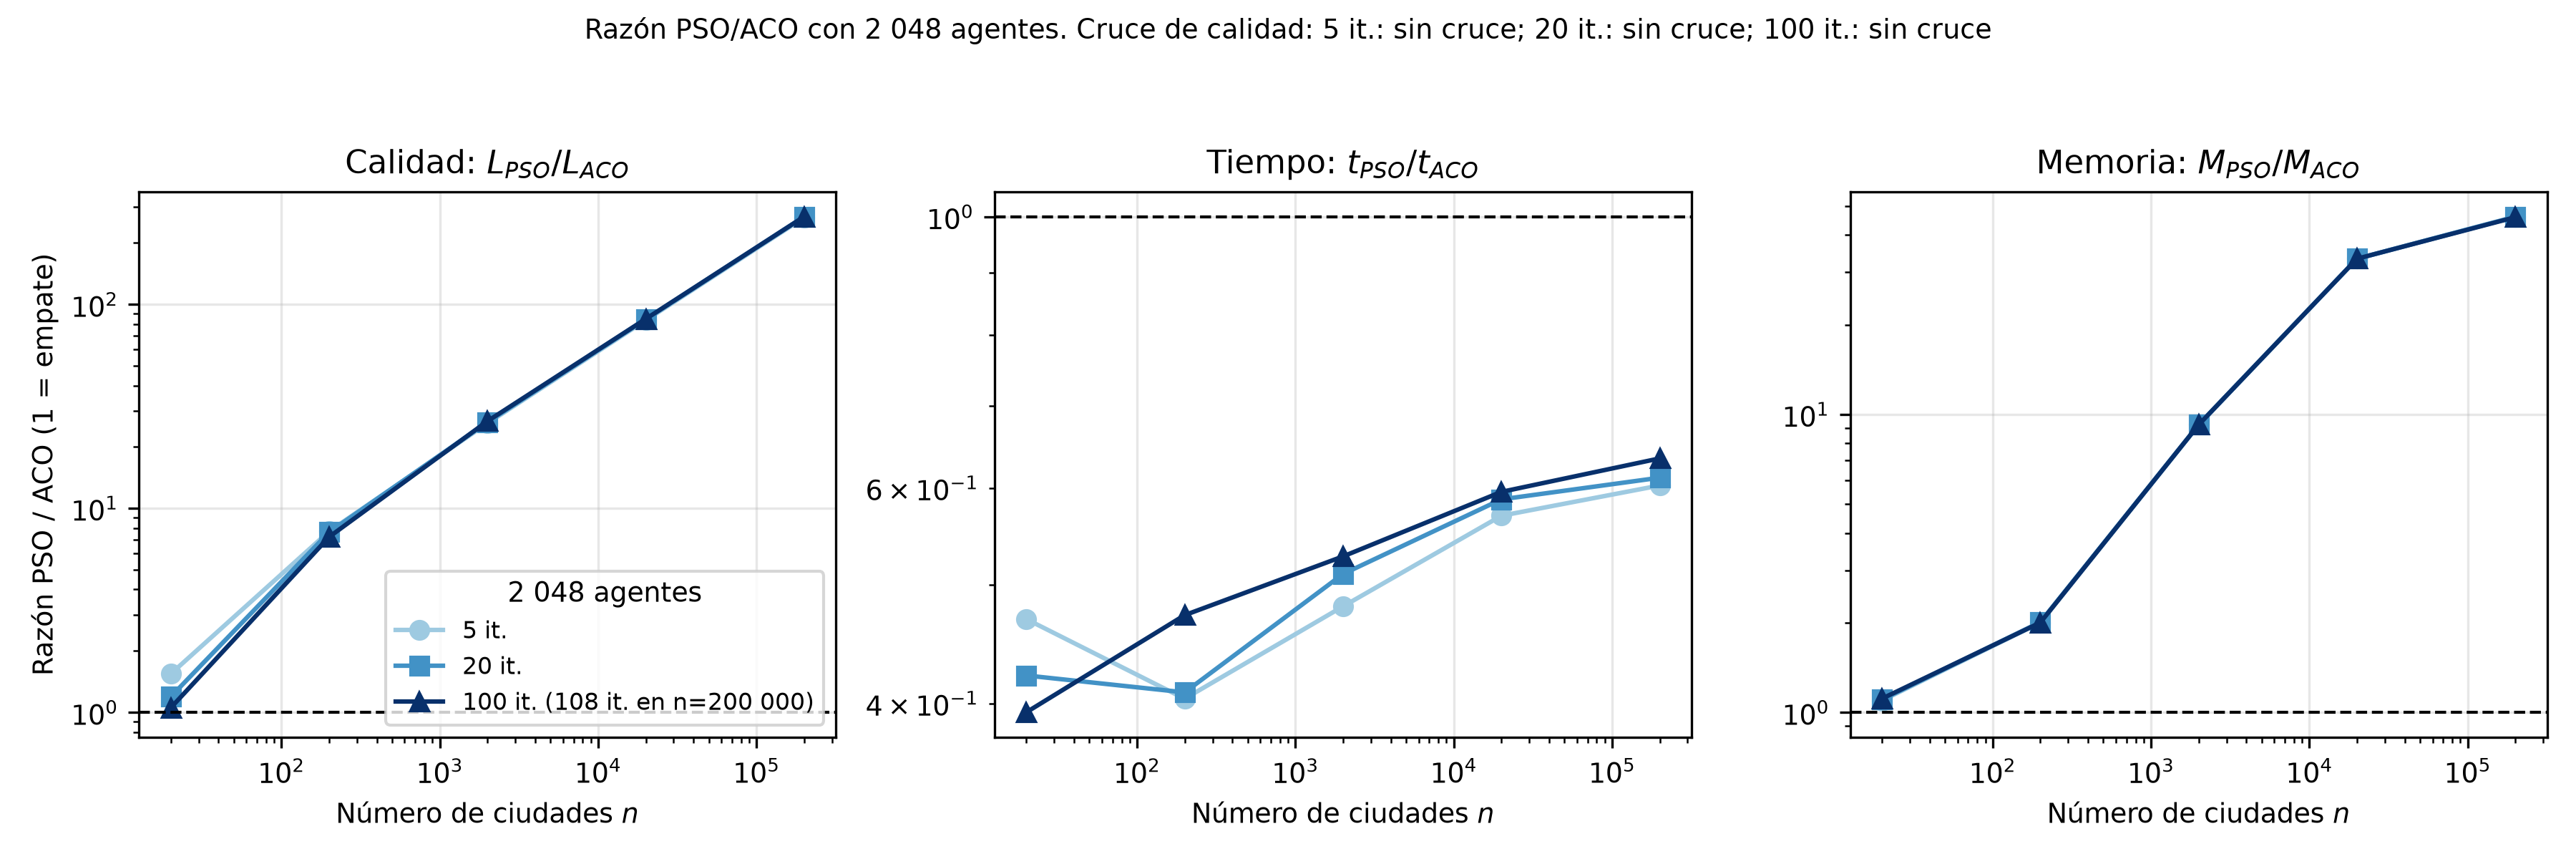
\includegraphics[width=\textwidth]{../figuras/barrido_razon_vs_n.png}
\caption{Razón PSO/ACO de calidad, tiempo y memoria en función de $n$, con 2\,048 agentes.
La línea punteada es la razón 1. En calidad y memoria la razón de PSO crece con $n$ sin cruzar el 1;
en tiempo se mantiene por debajo de 1.}
\label{fig:razon}
\end{figure}

\begin{figure}[H]\centering
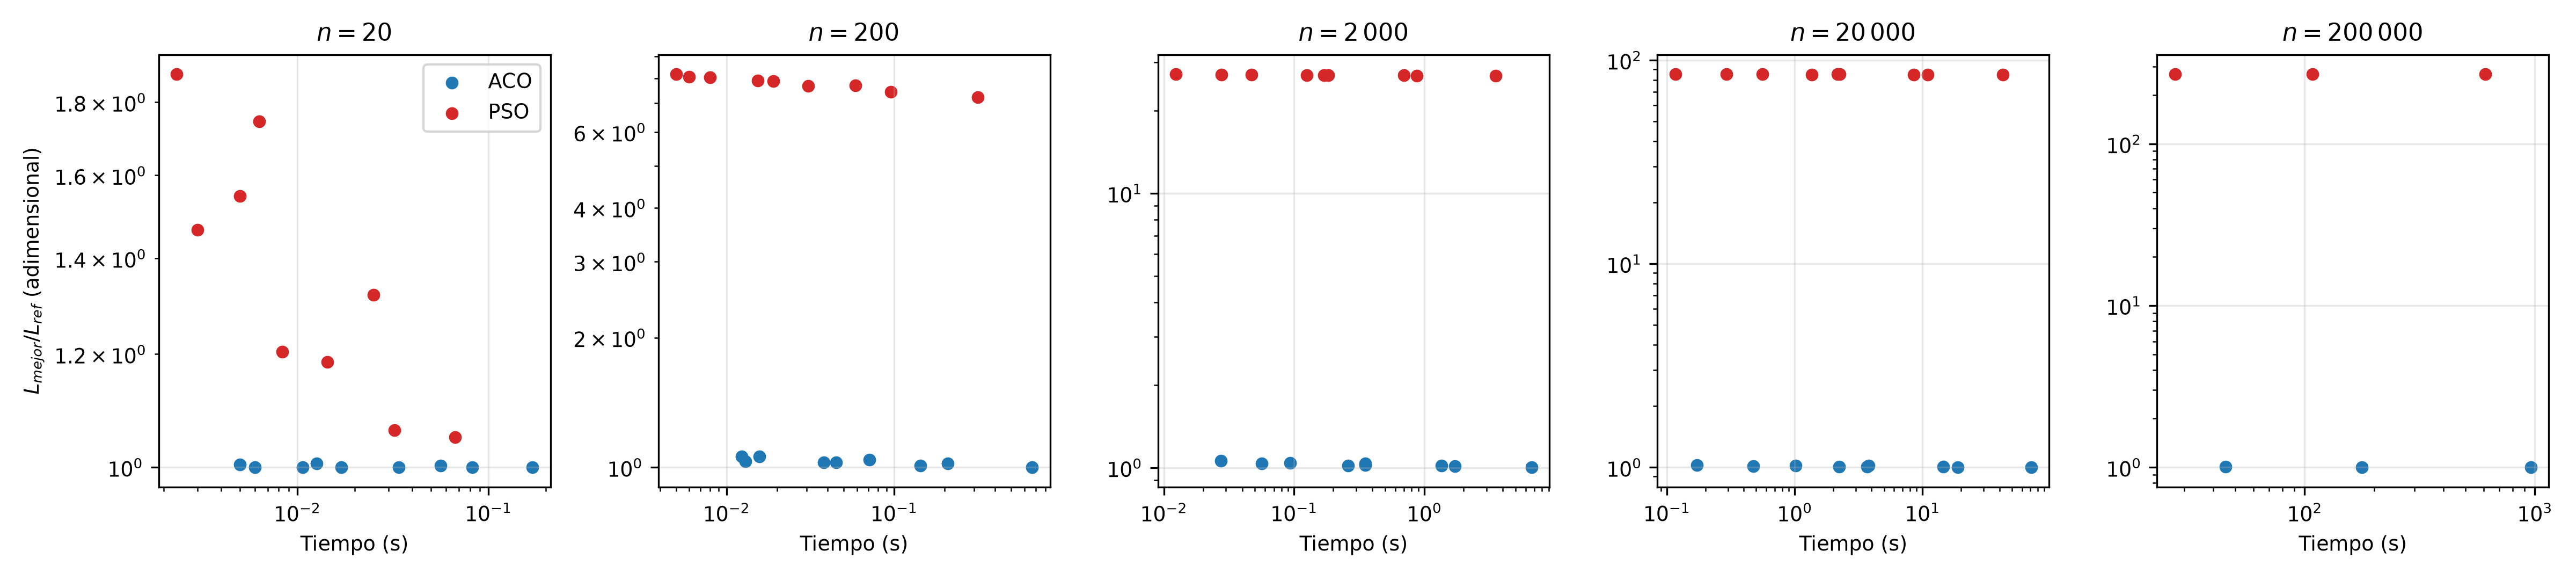
\includegraphics[width=\textwidth]{../figuras/barrido_calidad_vs_tiempo.png}
\caption{Calidad ($L_{mejor}/L_{ref}$) contra tiempo para las 9 configuraciones de cada $n$
(2 o 3 en $n=200\,000$; una de ellas con 108 it.). Con el mismo tiempo ACO queda más cerca de $L_{ref}$.}
\label{fig:calidad-tiempo}
\end{figure}

\begin{figure}[H]\centering
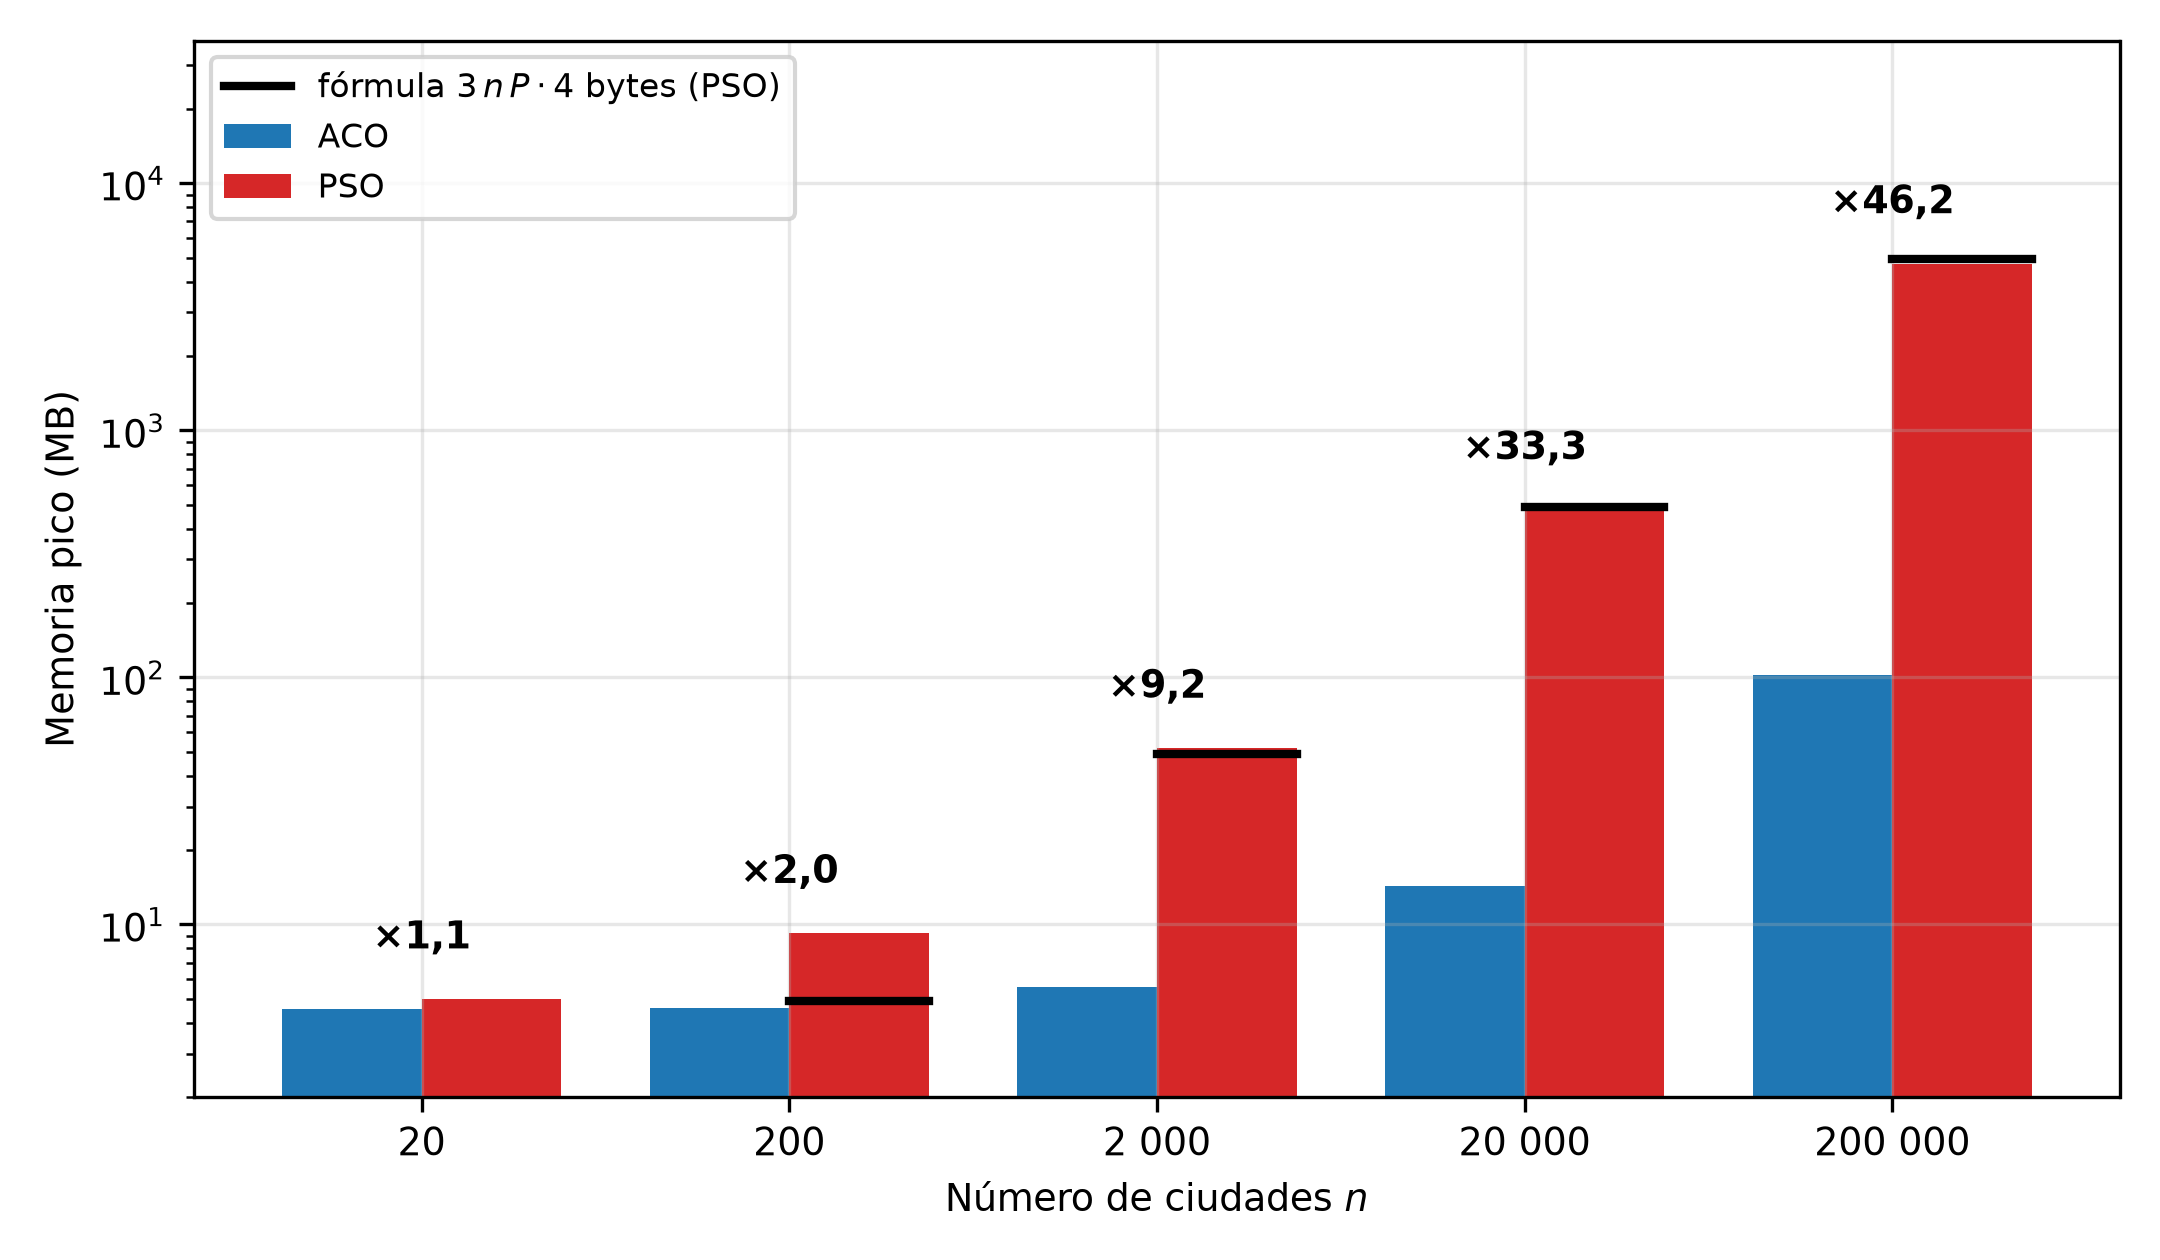
\includegraphics[width=0.62\textwidth]{../figuras/barrido_memoria.png}
\caption{Memoria pico contra agentes. Línea punteada: $3\,n\,P\cdot4$ bytes (PSO).}
\label{fig:memoria}
\end{figure}

\begin{figure}[H]\centering
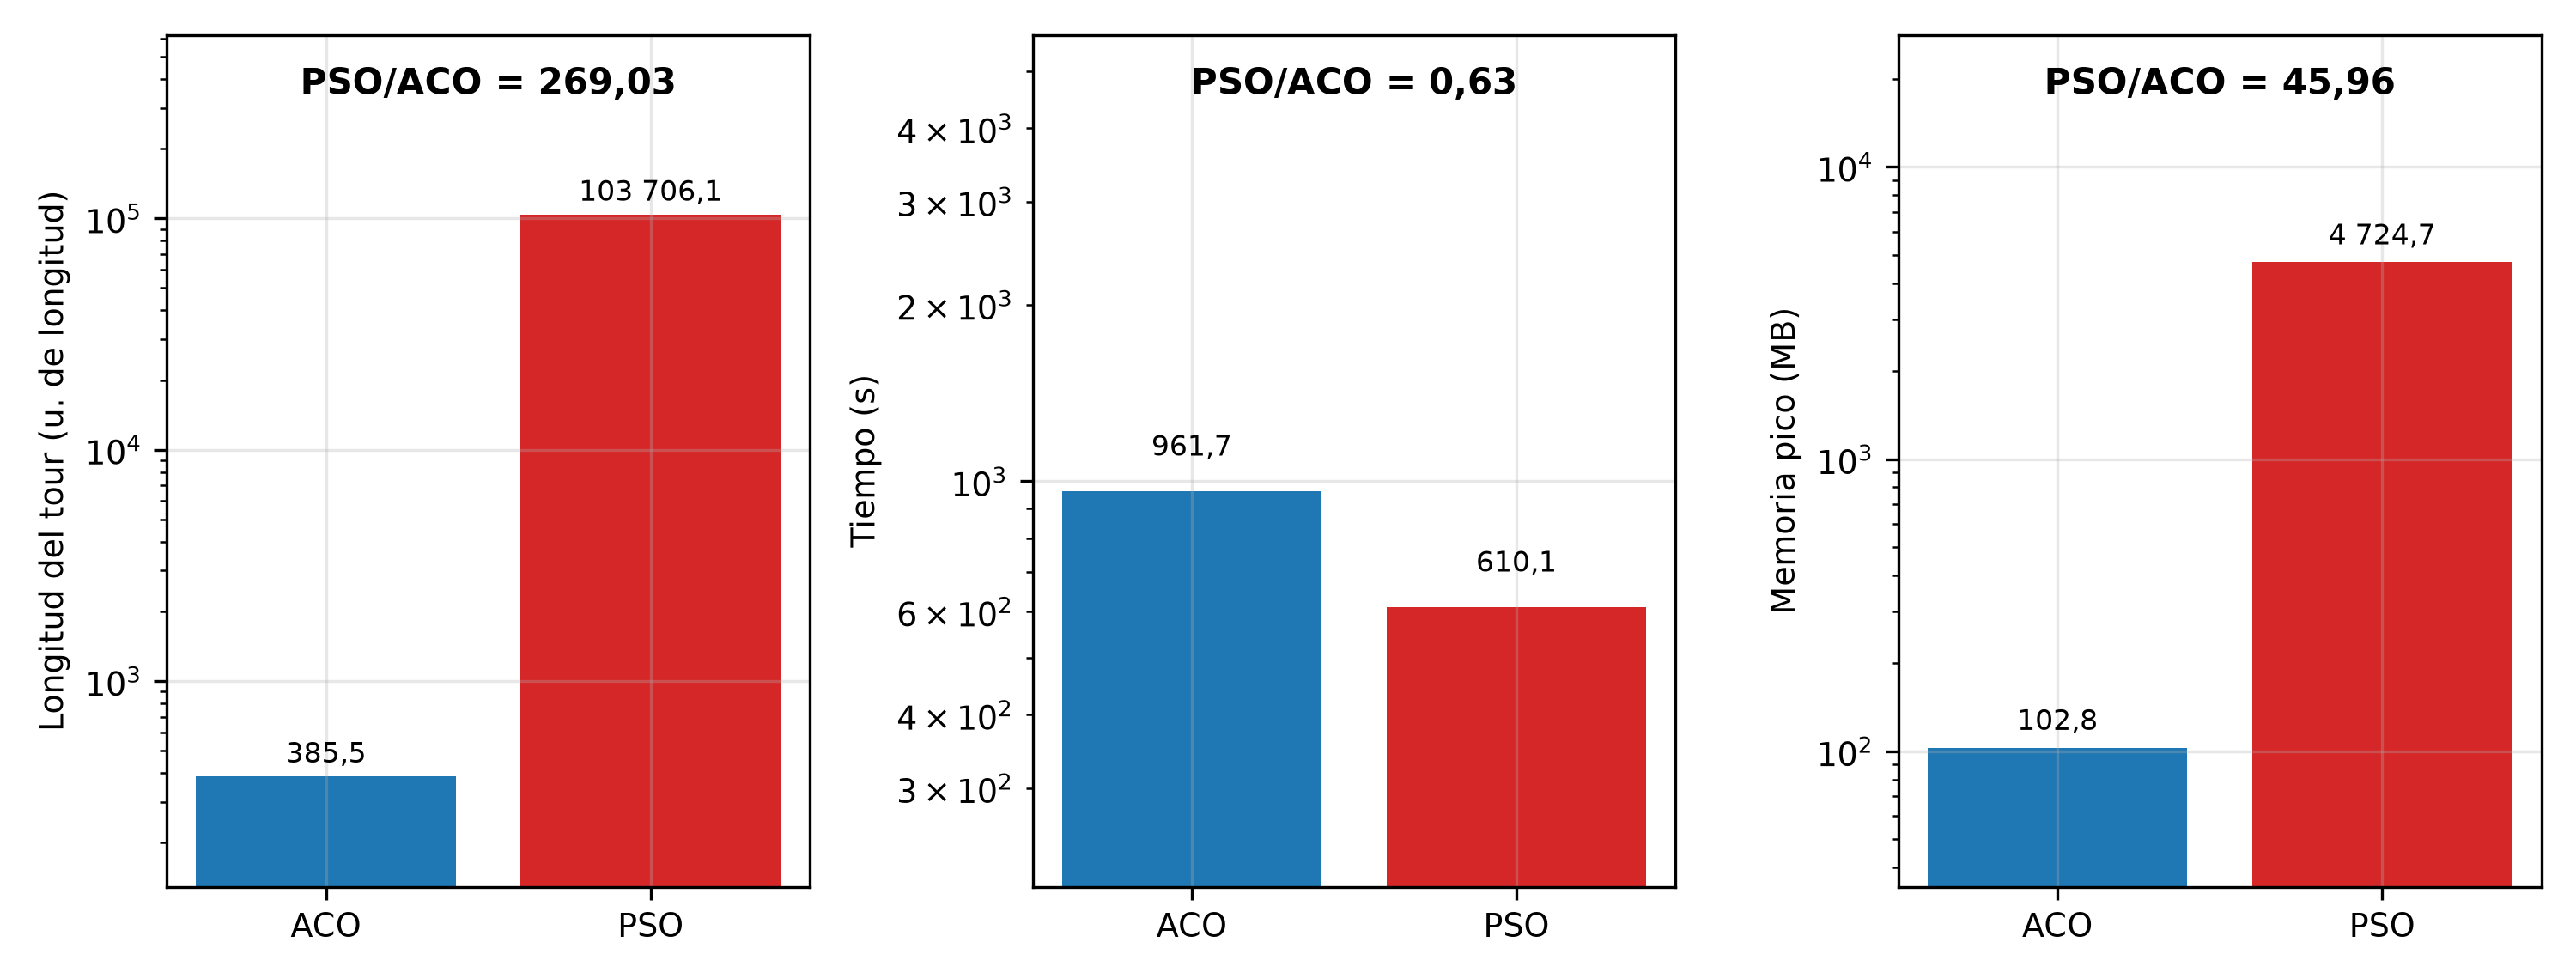
\includegraphics[width=0.85\textwidth]{../figuras/comparacion_P_igual_m.png}
\caption{$n=200\,000$, $P=m=2\,048$, 108 iteraciones: longitud, tiempo y memoria (escala logarítmica).}
\label{fig:igual-m}
\end{figure}

\subsection{Por qué PSO pesa}
Cada partícula guarda tres vectores de tamaño $n$ (posición, velocidad y mejor personal),
así que la memoria crece como $3\,n\,P\cdot4$ bytes (Figura~\ref{fig:memoria}).
En PSO con 2\,048 partículas la memoria pico medida dividida por $3\,n\,P\cdot4$ bytes vale 10,17 ($n=20$), 1,87 ($n=200$), 1,05 ($n=2\,000$), 0,97 ($n=20\,000$), 0,96 ($n=200\,000$); para $n\ge 2\,000$ la fórmula describe lo medido, y en $n$ pequeña domina la memoria base del proceso.

Además, cada evaluación exige ordenar $n$ claves, $O(n\log n)$, y cada iteración sortea $2n$
números aleatorios por partícula. ACO solo mantiene feromona sobre $n\cdot K$ aristas y no guarda
estado por hormiga entre iteraciones.

\subsection{Rutas}
\begin{figure}[H]\centering
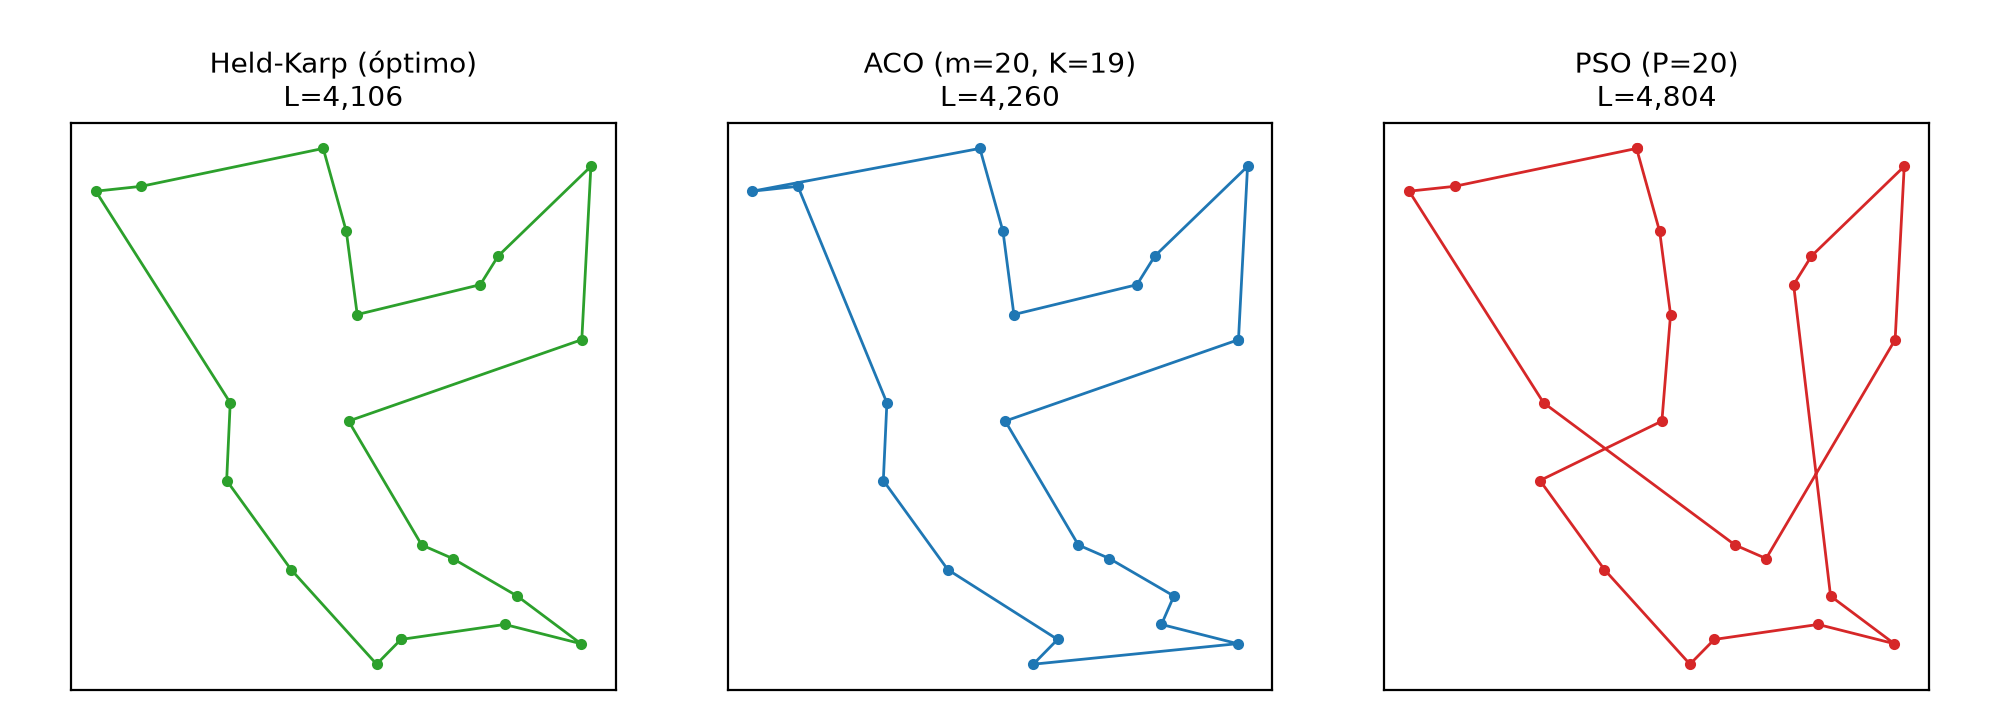
\includegraphics[width=0.48\textwidth]{../figuras/rutas_n20.png}\hfill
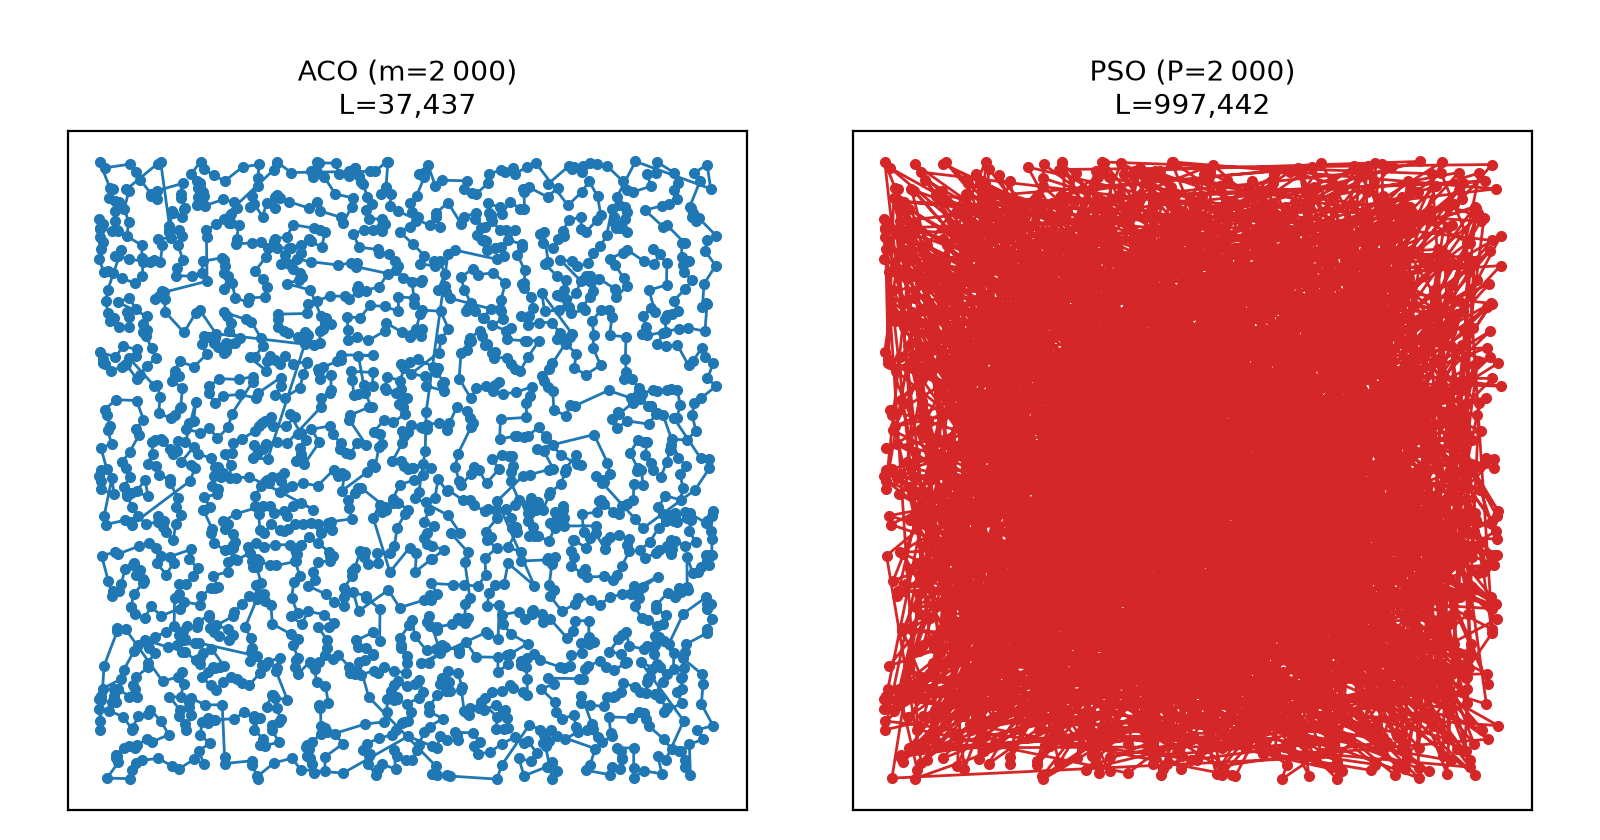
\includegraphics[width=0.48\textwidth]{../figuras/rutas_n2000.png}
\caption{Rutas en $n=20$ (Held-Karp, ACO, PSO) y $n=2\,000$ (ACO, PSO), ronda anterior.}
\end{figure}
\begin{figure}[H]\centering
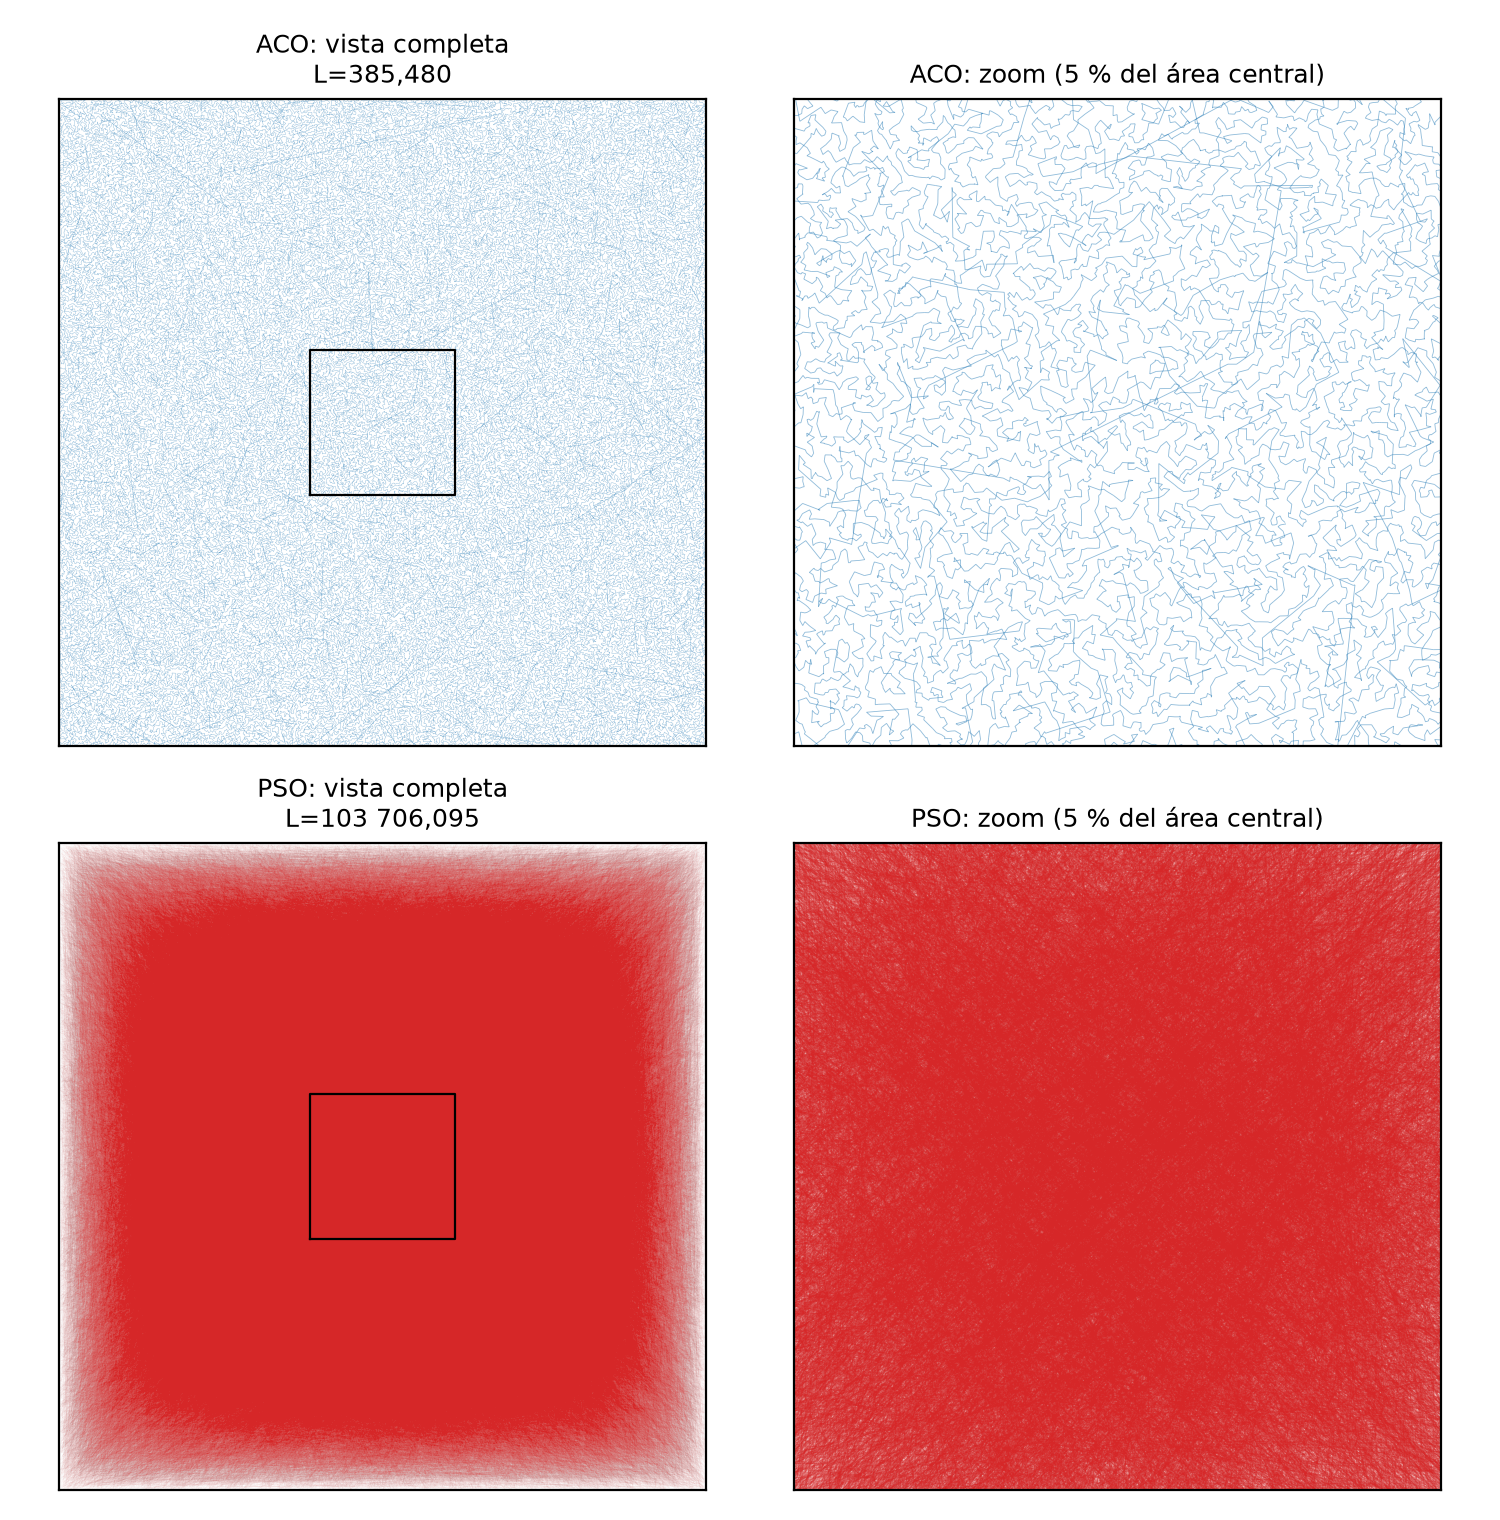
\includegraphics[width=0.75\textwidth]{../figuras/rutas_n200000.png}
\caption{Rutas en $n=200\,000$ (ACO y PSO, $P=m=2\,048$, 108 it.).}
\end{figure}

\subsection{Conclusiones de la comparación}
\begin{itemize}
\item \textbf{Calidad: ACO es mejor en todos los casos medidos.} Con 2\,048 agentes ACO obtiene menor $L_{mejor}$ en 15 de 15 combinaciones de $n$ e iteraciones, y en las 36 configuraciones emparejadas (mismo $n$, agentes e iteraciones; $n\le20\,000$) gana en 36 de 36. En $n=20$ ACO llega al óptimo de Held-Karp ($L/L_{ref}=1,000$ con 2\,048 agentes), mientras PSO queda 5,0\,\% por encima con 100 it. y 54,8\,\% con 5 it. En los demás $n$ ACO queda como máximo 3,4\,\% sobre la mejor longitud conocida, mientras que el tour de PSO es 7,2, 26,7, 84,8 y 269,0 veces más largo en $n=200$, 2\,000, 20\,000 y 200\,000.
\item \textbf{Dependencia de $n$: no hay cruce en el rango probado ($n=20$ a $n=200\,000$), y la brecha crece con $n$.} La razón $L_{PSO}/L_{ACO}$ con 2\,048 agentes y 100 it. (108 en $n=200\,000$) es 1,05 en $n=20$, 7,23 en $n=200$, 26,73 en $n=2\,000$, 84,80 en $n=20\,000$, 269,03 en $n=200\,000$: se multiplica por 256 entre $n=20$ y $n=200\,000$. No existe un tamaño de los probados en que PSO sea preferible por calidad; incluso donde la brecha es menor ($n=20$), ACO ya está en el óptimo.
\item \textbf{Tiempo: PSO es más rápido en todas las configuraciones emparejadas, pero su ventaja es menor que su desventaja de calidad.} PSO tarda entre 0,39 y 0,68 veces lo que ACO (ahorra entre 32\,\% y 61\,\% del tiempo); la razón mediana sube con $n$: 0,47 en $n=20$, 0,43 en $n=200$, 0,50 en $n=2\,000$, 0,60 en $n=20\,000$ y 0,63 en $n=200\,000$ (108 it.). En esta última instancia ACO usa 961,7 s para llegar a 385,5 y PSO 610,1 s para llegar a 103\,706: los 351,6 s que ahorra PSO no compensan un tour 269 veces más largo.
\item \textbf{Memoria: PSO usa más en todo el rango y la diferencia crece con $n$.} La razón $M_{PSO}/M_{ACO}$ con 2\,048 agentes es 1,1 en $n=20$, 2,0 en $n=200$, 9,2 en $n=2\,000$, 33,3 en $n=20\,000$, 46,2 en $n=200\,000$. En $n=200\,000$ PSO ocupa 4,7 GB y ACO 0,10 GB. La memoria de PSO sigue $3\,n\,P\cdot4$ bytes (tres vectores por partícula), por lo que con $P=20\,000$ partículas en $n=200\,000$ requeriría $\approx$48 GB y no cabe en el equipo (15,88 GB); ACO no guarda estado por hormiga entre iteraciones y su memoria casi no depende de los agentes.
\item \textbf{A igual tiempo ACO también gana.} Con el tiempo máximo común de cada $n$ ($T$), la mejor configuración de ACO y la de PSO alcanzan $L/L_{ref}$: $n=20$ ($T=0,07$ s): ACO 1,000, PSO 1,050; $n=200$ ($T=0,32$ s): ACO 1,009, PSO 7,236; $n=2\,000$ ($T=3,53$ s): ACO 1,010, PSO 26,806; $n=20\,000$ ($T=42,38$ s): ACO 1,001, PSO 84,844; $n=200\,000$ ($T=610,08$ s): ACO 1,002, PSO 269,031. Además, en 31 de 39 configuraciones de PSO existe una de ACO con tiempo y longitud menores o iguales.
\item \textbf{Veredicto.} ACO es la mejor opción para este TSP en calidad y en memoria en todo el rango probado ($n=20$ a $n=200\,000$); PSO solo gana en tiempo (0,39--0,68 veces el de ACO), una ventaja que no cambia el resultado al comparar a igual tiempo. La diferencia no depende del tamaño en el sentido del ganador, pero sí en su magnitud: es pequeña en $n=20$ y de más de dos órdenes de magnitud en $n=200\,000$.
\item \emph{Límites:} PSO con parámetros fijos ($w=0{,}7$, $c_1=c_2=1{,}5$) y sin búsqueda local; los resultados valen para esta implementación.
\end{itemize}



\section{Conclusiones}
\begin{enumerate}
\item PSO con claves aleatorias converge en instancias pequeñas ($n=20$), pero su calidad relativa a ACO empeora al crecer $n$, sin cruce en el rango probado ($n=20$ a $n=200\,000$).
\item PSO es más rápido por corrida en todas las configuraciones emparejadas, pero usa mucha más memoria, que crece como $3\,n\,P\cdot4$ bytes; con el mismo tiempo, ACO llega a mejor calidad (sección~\ref{sec:comparacion}).
\item Para TSP a esta escala, ACO (lista de $K$ candidatas y feromona por arista) es la opción superior; PSO con claves aleatorias, parámetros fijos y sin búsqueda local no está adaptado a este problema, y los resultados valen para esta implementación.
\end{enumerate}

\appendix
\section{Resultados completos del barrido}
\begin{table}[H]\centering
\caption{ACO vs. PSO, 9 configuraciones por $n$ (media $\pm$ desv. de 3 semillas).}
\footnotesize
\resizebox{\textwidth}{!}{%
\begin{tabular}{rrrrrrrrr}\toprule
\rowcolor{gray!25}
$n$ & Agentes & It. & $L$ ACO & $L$ PSO & $t$ ACO (s) & $t$ PSO (s) & Mem. ACO (MB) & Mem. PSO (MB) \\\midrule
20 & 50 & 5 & 4,556 $\pm$ 0,378 & 8,512 $\pm$ 0,519 & 0,01 & 0,00 & 4,5 & 4,5 \\
20 & 50 & 20 & 4,563 $\pm$ 0,348 & 7,884 $\pm$ 0,087 & 0,01 & 0,01 & 4,5 & 4,5 \\
20 & 50 & 100 & 4,549 $\pm$ 0,372 & 5,987 $\pm$ 0,596 & 0,06 & 0,02 & 4,5 & 4,5 \\
20 & 500 & 5 & 4,535 $\pm$ 0,359 & 6,616 $\pm$ 0,154 & 0,01 & 0,00 & 4,5 & 4,6 \\
20 & 500 & 20 & 4,535 $\pm$ 0,359 & 5,448 $\pm$ 0,160 & 0,02 & 0,01 & 4,5 & 4,6 \\
20 & 500 & 100 & 4,535 $\pm$ 0,359 & 4,822 $\pm$ 0,580 & 0,08 & 0,03 & 4,5 & 4,6 \\
20 & 2\,048 & 5 & 4,535 $\pm$ 0,359 & 6,993 $\pm$ 0,372 & 0,01 & 0,01 & 4,6 & 5,0 \\
20 & 2\,048 & 20 & 4,535 $\pm$ 0,359 & 5,401 $\pm$ 1,002 & 0,03 & 0,01 & 4,5 & 5,0 \\
20 & 2\,048 & 100 & 4,535 $\pm$ 0,359 & 4,768 $\pm$ 0,575 & 0,17 & 0,07 & 4,5 & 5,0 \\
200 & 50 & 5 & 12,087 $\pm$ 0,105 & 93,352 $\pm$ 1,640 & 0,01 & 0,01 & 4,6 & 4,6 \\
200 & 50 & 20 & 12,090 $\pm$ 0,156 & 91,779 $\pm$ 0,527 & 0,02 & 0,01 & 4,6 & 4,6 \\
200 & 50 & 100 & 11,907 $\pm$ 0,123 & 87,767 $\pm$ 1,508 & 0,07 & 0,03 & 4,6 & 4,6 \\
200 & 500 & 5 & 11,783 $\pm$ 0,231 & 91,934 $\pm$ 1,887 & 0,01 & 0,01 & 4,6 & 5,7 \\
200 & 500 & 20 & 11,714 $\pm$ 0,110 & 89,902 $\pm$ 1,545 & 0,05 & 0,02 & 4,6 & 5,7 \\
200 & 500 & 100 & 11,669 $\pm$ 0,071 & 85,006 $\pm$ 4,643 & 0,21 & 0,10 & 4,6 & 5,7 \\
200 & 2\,048 & 5 & 11,712 $\pm$ 0,130 & 90,261 $\pm$ 1,111 & 0,04 & 0,02 & 4,6 & 9,2 \\
200 & 2\,048 & 20 & 11,526 $\pm$ 0,083 & 87,975 $\pm$ 2,186 & 0,14 & 0,06 & 4,6 & 9,2 \\
200 & 2\,048 & 100 & 11,423 $\pm$ 0,178 & 82,645 $\pm$ 4,606 & 0,67 & 0,32 & 4,6 & 9,2 \\
2\,000 & 50 & 5 & 39,539 $\pm$ 0,249 & 1\,014,505 $\pm$ 11,780 & 0,03 & 0,01 & 5,6 & 5,9 \\
2\,000 & 50 & 20 & 38,669 $\pm$ 0,040 & 1\,009,993 $\pm$ 8,551 & 0,06 & 0,03 & 5,6 & 6,0 \\
2\,000 & 50 & 100 & 38,021 $\pm$ 0,033 & 1\,004,623 $\pm$ 8,546 & 0,26 & 0,13 & 5,6 & 6,0 \\
2\,000 & 500 & 5 & 38,893 $\pm$ 0,064 & 1\,008,236 $\pm$ 7,713 & 0,09 & 0,05 & 5,6 & 16,3 \\
2\,000 & 500 & 20 & 38,219 $\pm$ 0,255 & 1\,006,244 $\pm$ 4,922 & 0,35 & 0,18 & 5,6 & 16,3 \\
2\,000 & 500 & 100 & 37,719 $\pm$ 0,410 & 1\,002,152 $\pm$ 5,770 & 1,72 & 0,88 & 5,6 & 16,3 \\
2\,000 & 2\,048 & 5 & 38,605 $\pm$ 0,118 & 1\,007,924 $\pm$ 7,987 & 0,35 & 0,17 & 5,6 & 51,7 \\
2\,000 & 2\,048 & 20 & 38,018 $\pm$ 0,469 & 1\,005,522 $\pm$ 6,900 & 1,36 & 0,69 & 5,6 & 51,7 \\
2\,000 & 2\,048 & 100 & 37,452 $\pm$ 0,213 & 1\,000,979 $\pm$ 3,988 & 6,69 & 3,53 & 5,6 & 51,7 \\
20\,000 & 50 & 5 & 123,894 $\pm$ 0,135 & 10\,326,994 $\pm$ 41,975 & 0,17 & 0,12 & 14,3 & 19,2 \\
20\,000 & 50 & 20 & 122,518 $\pm$ 0,399 & 10\,322,464 $\pm$ 41,156 & 0,47 & 0,29 & 14,3 & 19,2 \\
20\,000 & 50 & 100 & 121,663 $\pm$ 0,617 & 10\,300,515 $\pm$ 20,671 & 2,23 & 1,37 & 14,3 & 19,2 \\
20\,000 & 500 & 5 & 123,386 $\pm$ 0,545 & 10\,315,746 $\pm$ 30,913 & 1,01 & 0,56 & 14,3 & 122,2 \\
20\,000 & 500 & 20 & 122,076 $\pm$ 0,604 & 10\,306,164 $\pm$ 37,608 & 3,68 & 2,24 & 14,3 & 122,2 \\
20\,000 & 500 & 100 & 121,231 $\pm$ 0,260 & 10\,298,055 $\pm$ 30,671 & 18,97 & 10,96 & 14,3 & 122,2 \\
20\,000 & 2\,048 & 5 & 123,380 $\pm$ 0,313 & 10\,303,629 $\pm$ 42,434 & 3,79 & 2,16 & 14,3 & 476,6 \\
20\,000 & 2\,048 & 20 & 121,808 $\pm$ 0,407 & 10\,287,972 $\pm$ 31,052 & 14,57 & 8,56 & 14,3 & 476,6 \\
20\,000 & 2\,048 & 100 & 121,162 $\pm$ 0,462 & 10\,274,472 $\pm$ 42,107 & 71,15 & 42,38 & 14,3 & 476,6 \\
200\,000 & 2\,048 & 5 & 390,059 $\pm$ 0,512 & 103\,803,161 $\pm$ 49,981 & 45,29 & 27,30 & 102,4 & 4\,726,1 \\
200\,000 & 2\,048 & 20 & 386,061 $\pm$ 0,335 & 103\,787,889 $\pm$ 60,275 & 176,99 & 108,27 & 102,5 & 4\,726,0 \\
\bottomrule\end{tabular}%
}

\end{table}

\begin{figure}[H]\centering
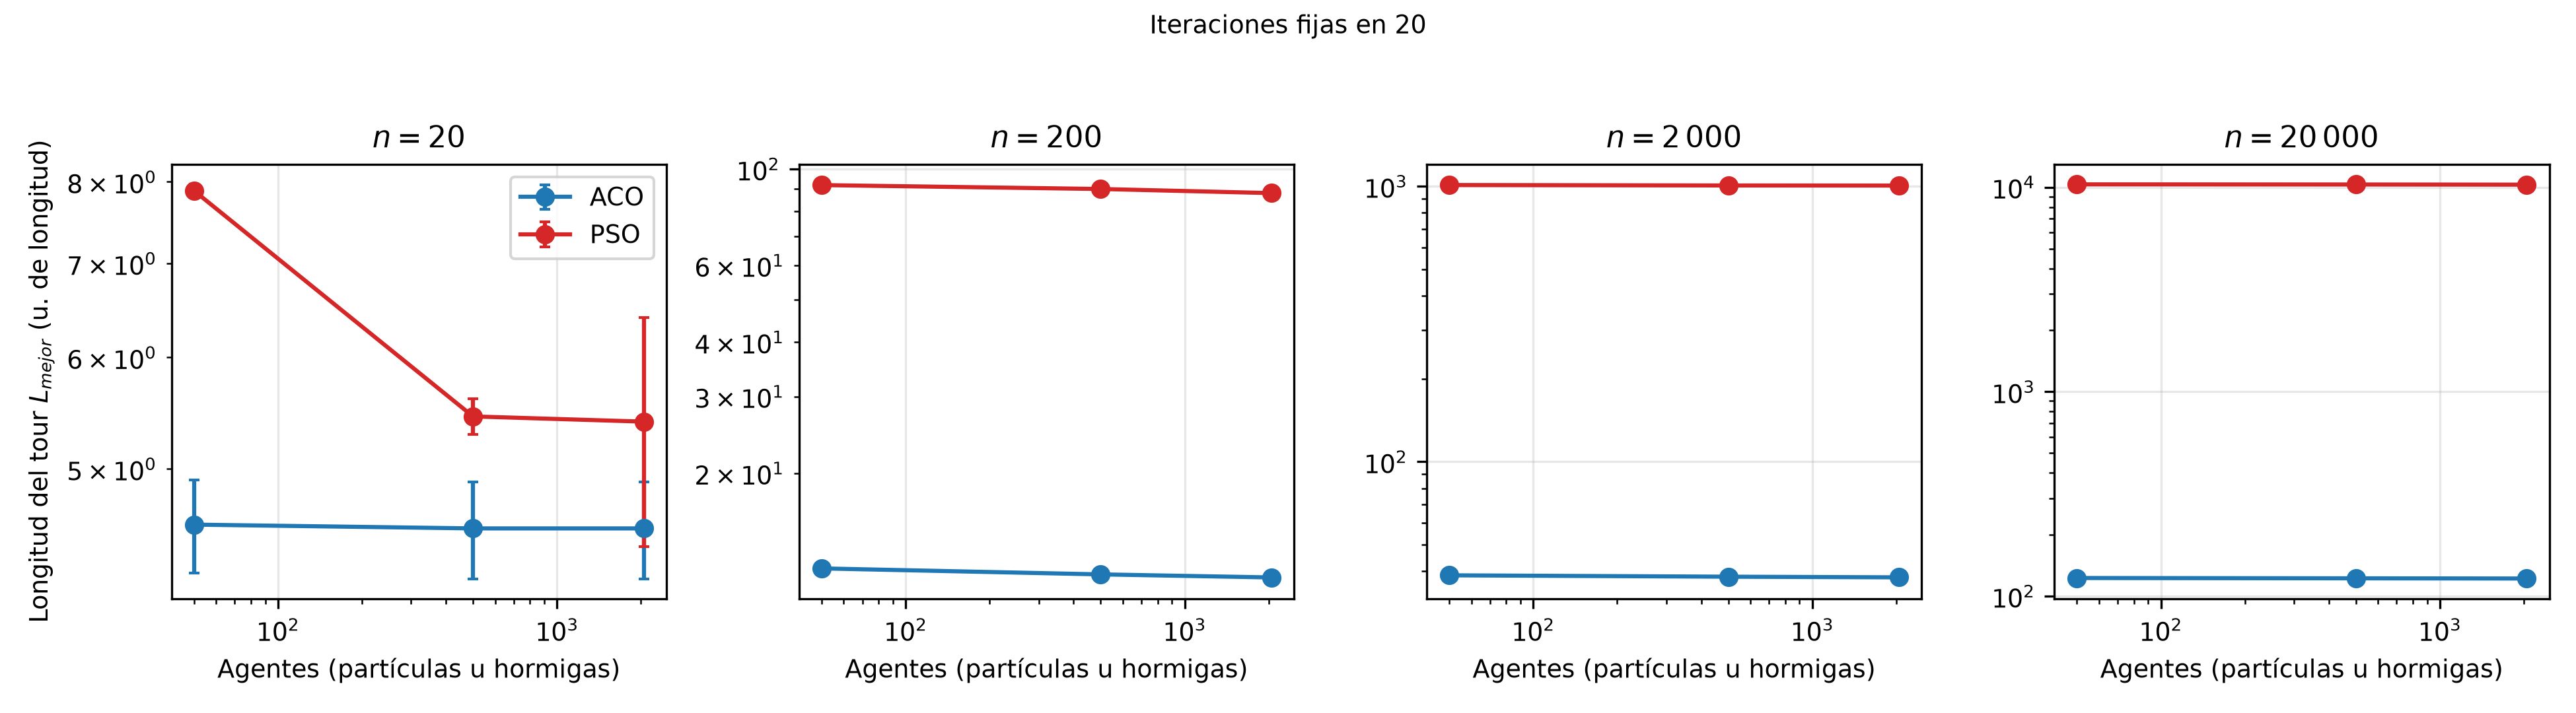
\includegraphics[width=\textwidth]{../figuras/barrido_calidad_agentes.png}
\caption{$L_{mejor}$ contra agentes, con 20 iteraciones.}
\end{figure}
\begin{figure}[H]\centering
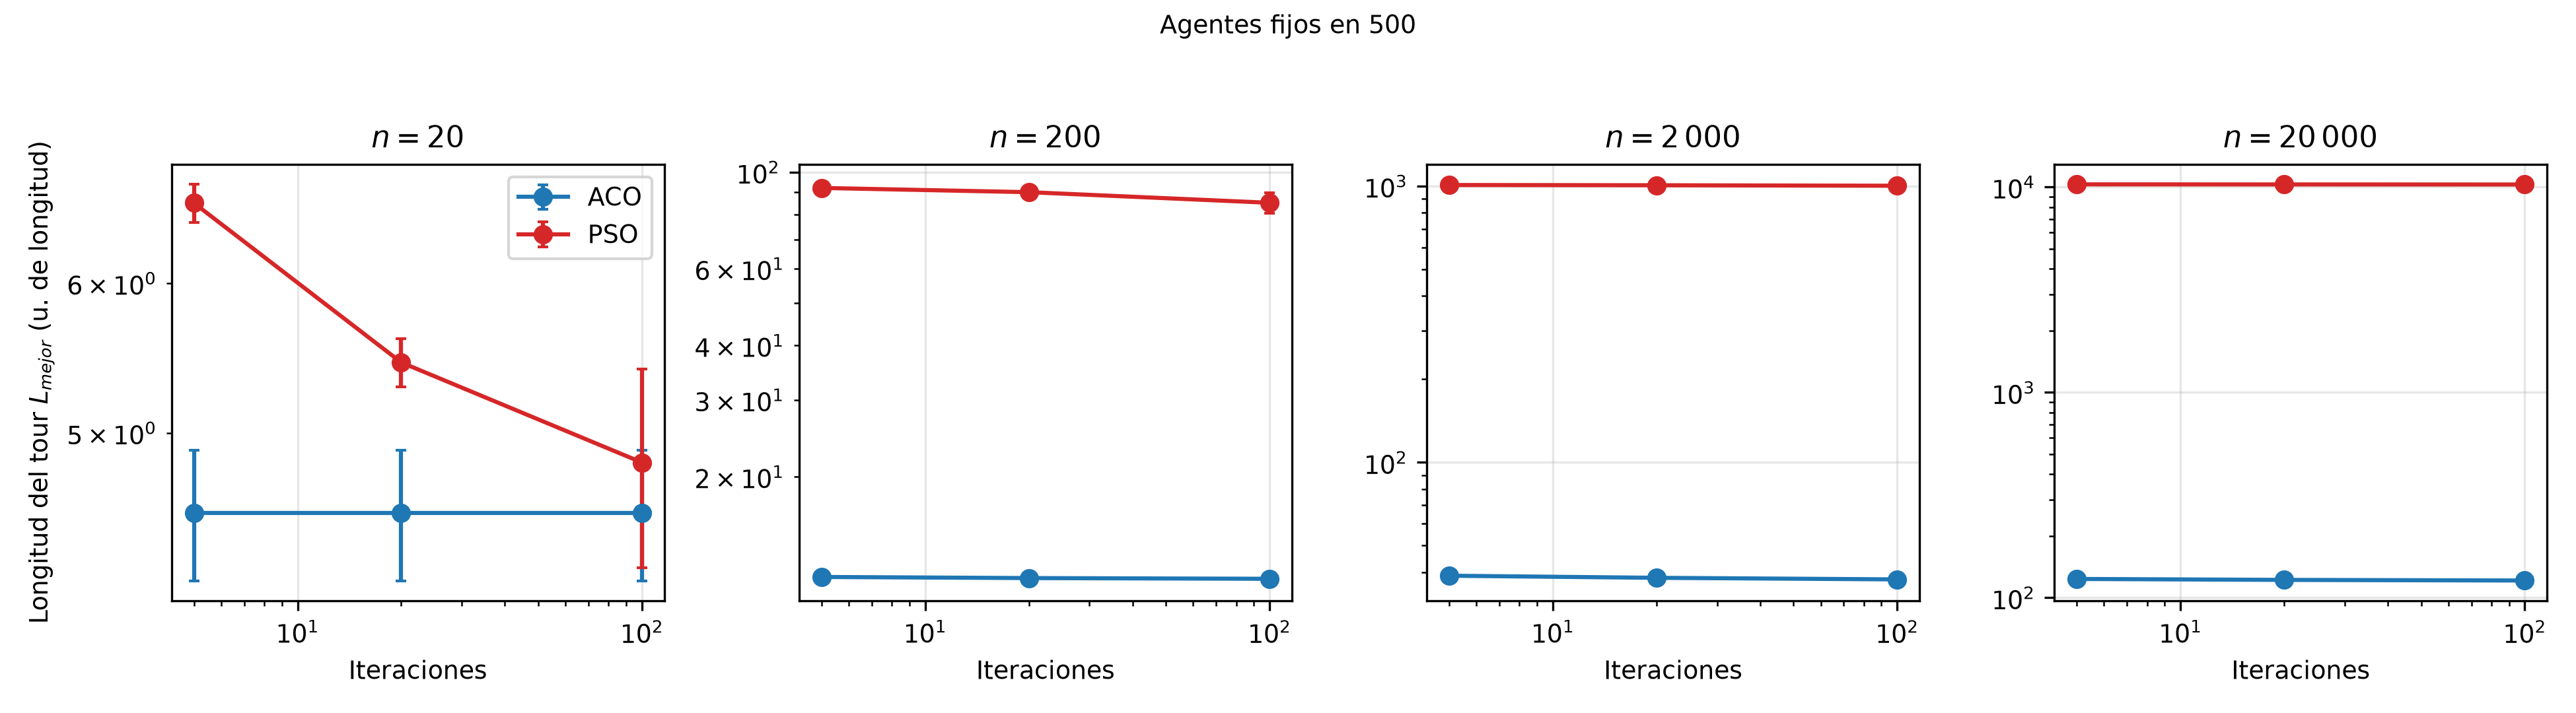
\includegraphics[width=\textwidth]{../figuras/barrido_calidad_iteraciones.png}
\caption{$L_{mejor}$ contra iteraciones, con 500 agentes.}
\end{figure}
\begin{figure}[H]\centering
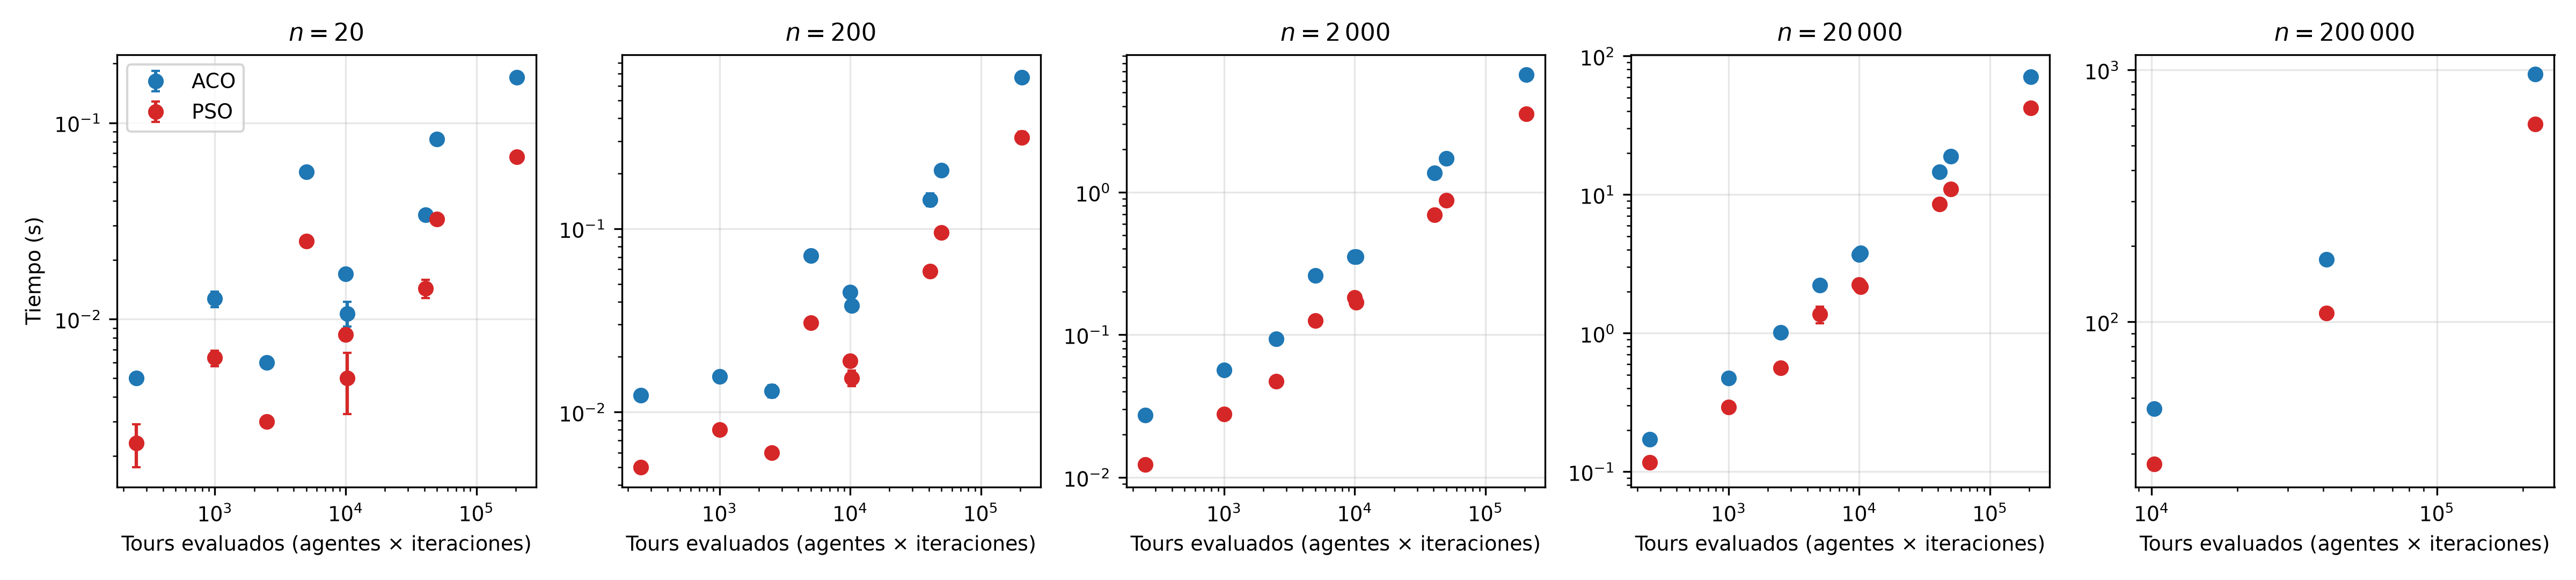
\includegraphics[width=\textwidth]{../figuras/barrido_tiempo.png}
\caption{Tiempo contra tours evaluados (agentes $\times$ iteraciones).}
\end{figure}
\begin{figure}[H]\centering
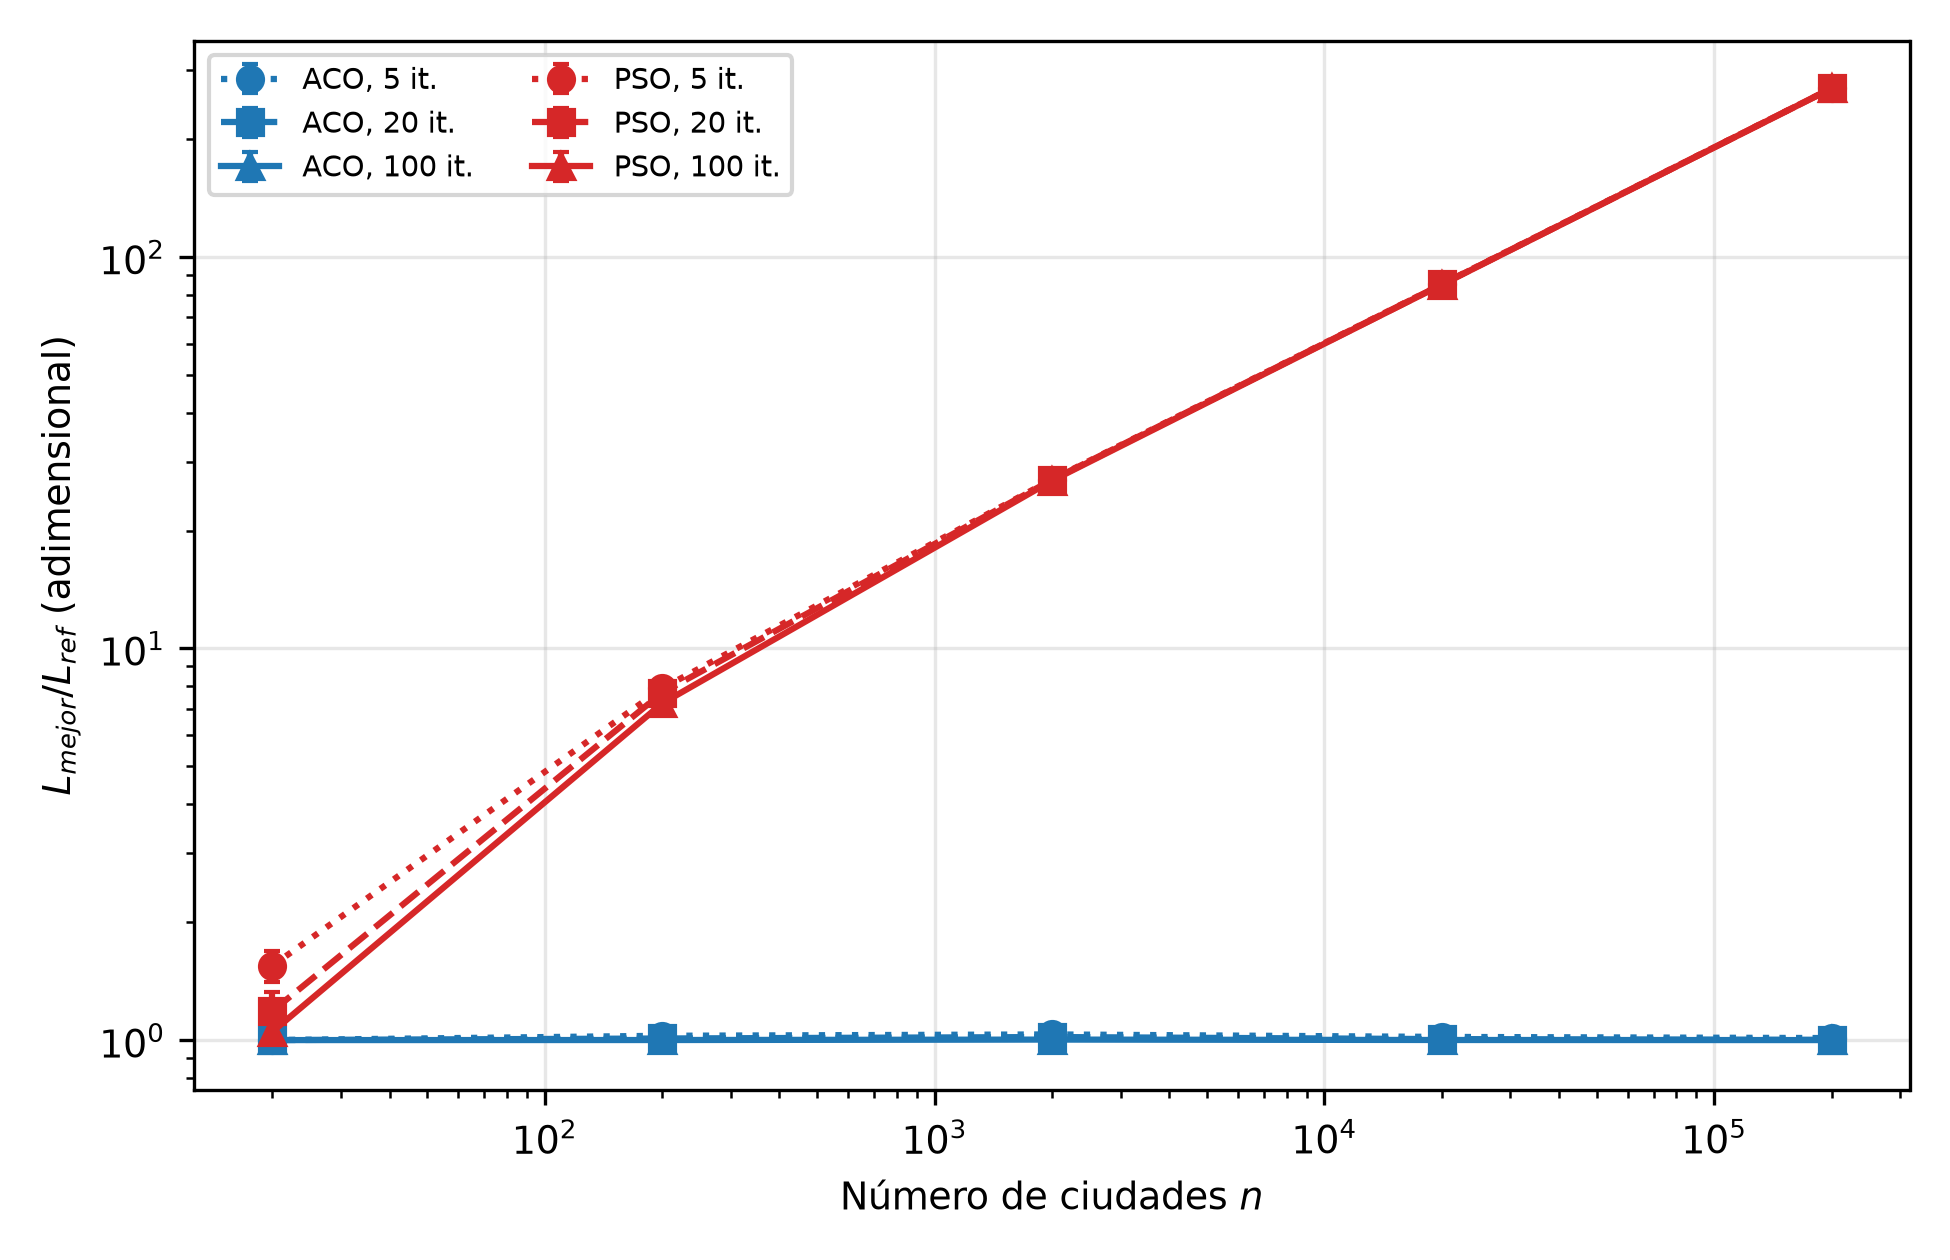
\includegraphics[width=0.6\textwidth]{../figuras/barrido_calidad_vs_n.png}
\caption{$L_{mejor}/L_{ref}$ contra $n$ con 2\,048 agentes ($L_{ref}$: óptimo de Held-Karp en $n=20$; en los demás $n$, la mejor longitud medida).}
\end{figure}


\end{document}
